%%%%%%%%%%%%%%%%%%%%%%%%%%%%%%%%%%%%%%%%%%%%%%%%%
% This tex file uses minted package.
% Do not compile if Pygments highlighter for 
% minted is not installed. 
% Use admin to compile this file.
% External data file is provided in the code/ folder.
%%%%%%%%%%%%%%%%%%%%%%%%%%%%%%%%%%%%%%%%%%%%%%%%%

\documentclass[12pt,a4paper]{article}
\usepackage{amsmath,amscd,amsbsy,amssymb,latexsym,url,bm,amsthm}
\usepackage{epsfig,graphicx,subfigure}
\usepackage{enumitem,balance}
\usepackage{wrapfig}
\usepackage{mathrsfs,euscript}
\usepackage[usenames]{xcolor}
\usepackage{hyperref}
\usepackage[vlined,ruled,linesnumbered]{algorithm2e}
\hypersetup{colorlinks=true,linkcolor=black}

\newtheorem{theorem}{Theorem}
\newtheorem{lemma}[theorem]{Lemma}
\newtheorem{proposition}[theorem]{Proposition}
\newtheorem{corollary}[theorem]{Corollary}
\newtheorem{exercise}{Exercise}
\newtheorem*{solution}{Solution}
\newtheorem{definition}{Definition}
\theoremstyle{definition}

\renewcommand{\thefootnote}{\fnsymbol{footnote}}

\newcommand{\postscript}[2]
 {\setlength{\epsfxsize}{#2\hsize}
  \centerline{\epsfbox{#1}}}

\renewcommand{\baselinestretch}{1.0}

\setlength{\oddsidemargin}{-0.365in}
\setlength{\evensidemargin}{-0.365in}
\setlength{\topmargin}{-0.3in}
\setlength{\headheight}{0in}
\setlength{\headsep}{0in}
\setlength{\textheight}{10.1in}
\setlength{\textwidth}{7in}
\makeatletter \renewenvironment{proof}[1][Proof] {\par\pushQED{\qed}\normalfont\topsep6\p@\@plus6\p@\relax\trivlist\item[\hskip\labelsep\bfseries#1\@addpunct{.}]\ignorespaces}{\popQED\endtrivlist\@endpefalse} \makeatother
\makeatletter
\renewenvironment{solution}[1][Solution] {\par\pushQED{\qed}\normalfont\topsep6\p@\@plus6\p@\relax\trivlist\item[\hskip\labelsep\bfseries#1\@addpunct{.}]\ignorespaces}{\popQED\endtrivlist\@endpefalse} \makeatother

\usepackage{codeblock}
\usepackage{tikz}

\begin{document}
\noindent

%========================================================================
\noindent\framebox[\linewidth]{\shortstack[c]{
\Large{\textbf{Lab02-Divide and Conquer}}\vspace{1mm}\\
CS214-Algorithm and Complexity, Xiaofeng Gao, Spring 2021.}}
\begin{center}
\footnotesize{\color{red}$*$ If there is any problem, please contact TA Haolin Zhou. }

\footnotesize{\color{blue}$*$ Name: Zilong Li  \quad Student ID: 518070910095 \quad Email: logcreative-lzl@sjtu.edu.cn}
\end{center}

\begin{enumerate}
\item
    \textit{Recurrence examples.} Give asymptotic upper and lower bounds for $T(n)$ in each of the following recurrences. Assume that $T(n)$ is constant for sufficiently small $n$. Make your bounds as tight as possible.
\begin{enumerate}
	\item $T(n)=4 T(n / 3)+n \log n$
	\item $T(n)=4 T(n / 2)+n^{2} \sqrt{n}$
	\item $T(n)=T(n-1)+n$	
	\item $T(n)=2T(\lfloor \sqrt n\rfloor)+\log n$
\end{enumerate}
\begin{solution}
    \begin{enumerate}
        \item 
            \begin{align*}
                T(n) = 4 T(n / 3)+n \log n &= \sum_{i=0}^{\log_3 n}4^i \frac{n}{3^i}\log\frac{n}{3^i} \\&= \sum_{j=0}^{\log_3 n}\left(\frac{4}{3}\right)^{\log_3 n} \left(\frac{3}{4}\right)^j n\log\frac{n}{3^{\log_3 n-j}} \\
                &=\left(\frac{4}{3}\right)^{\log_3 n} n\log 3 \sum_{j=0}^{\log_3 n}j\left(\frac{3}{4}\right)^j \\
                &= \left(\frac{4}{3}\right)^{\log_3 n} n\log 3\cdot 4 \left[\sum_{j=1}^{\log_3 n}\left(\frac{3}{4}\right)^j - \log_3 n \cdot \left(\frac{3}{4}\right)^{(\log_3 n) +1}\right]\\
                &=12\left(\frac{4}{3}\right)^{\log_3 n} n\log 3 \cdot \left[1-\left(\frac{3}{4}\right)^{\log_3 n}\left(1+\frac{1}{4}\log_3 n \right)\right]\\
                &=12\log 3\cdot 4^{\log_3 n} - 12 n\log 3 - 3n\log n \text{ (lower bound)}\\
                &\leq 12\log 3\cdot n^{\log_3 4} = O(n^{\log_3 4}) \text{ (upper bound)}
            \end{align*}

        \item \begin{equation*}
            T(n) = 4 T(n / 2)+n^{2} \sqrt{n} = 4T\left(\frac{n}{2}\right) + n^{5/2}
        \end{equation*}
        According to the Master Theorem, $d=\frac{5}{2} > \log_b a = 2$, Then,
        \begin{equation*}
            T(n) = O(n^{5/2}) \text{ (upper bound)}
        \end{equation*}
        In fact, by the same deduction in the Master Theorem,
        \begin{equation*}
            T(n) = n^{5/2}\frac{1}{2^{5/2}-4} \approx 0.61 n^{5/2} = \Theta(n^{5/2}) \text{ (upper and lower bounds)}
        \end{equation*}
        \item \begin{align*}
            T(n) = \sum_{i=1}^n i &= \frac{n(n+1)}{2}&&\text{ (lower bound)}\\
            &= O(n^2)&&\text{ (upper bound)}
        \end{align*}
       
        \item \begin{equation*}
            T(n)=2T(\lfloor \sqrt n\rfloor)+\log n = 2T(1) + \sum_{i=0}^k 2^k \log n^{\frac{1}{2^k}} = 2T(1) + \sum_{i=0}^k \log n
        \end{equation*}
        To get the layer number $k$, the recurrence should stop when $\lfloor \sqrt n\rfloor=1$ for no further drop on the input. As a result,
        \begin{align*}
           \lfloor n^{1/2^{k}}\rfloor &< 4 \\
           n&< 2^{2^{k+1}}\\
           k&> \log_2 (\log_2 n - 1)
        \end{align*}
        \begin{align*}
            T(n)&=2T(1)+\log_2 (\log_2 n - 1)\log n\\
            &=\log_2 (\log_2 n - 1)\log n&&\text{ (lower bound)} \\
            &= O(\log\log\log n)&&\text{ (upper bound)}
        \end{align*}
    \end{enumerate}
    
\end{solution}
\item
\textit{Divide-and-conquer.} Given an integer array $A[1..n]$ and two integers $lower \le upper$, design an algorithm using \textbf{divide-and-conquer} method to count the number of ranges $(i,j)$ ($1 \leq i \leq j \leq n$) satisfying
$$
    lower \leq \sum_{k=i}^{j}{A[k]} \leq upper.
$$
\textbf{Example:}

Given $A = [1,-1,2]$, $lower = 1$, $upper = 2$, return 4.

The resulting four ranges are $(1,1)$, $(3,3)$, $(2,3)$ and $(1,3)$.

\begin{enumerate}
\item
Complete the implementation in the provided C/C++ source code {\color{blue}(The source code \emph{Code-Range.cpp} is attached on the course webpage)}.
\item
Write a recurrence for the running time of the algorithm and solve it by recurrence tree {\color{blue}(You can modify the figure sources \emph{Fig-RecurrenceTree.vsdx} or \emph{Fig-RecurrenceTree.pptx} to illustrate your derivation)}.
\item
Can we use the Master Theorem to solve the recurrence above? Please explain your answer.
\end{enumerate}
\begin{solution}
\begin{enumerate}
    \item The implementation is shown as follows:
    \fname{Code-Range.cpp}
    \inputminted[]{cpp}{code/Code-Range.cpp} % Comment the line if package minted is not supported.
    
    \item Because the modified binary search is worth the time complexity of $\Theta(\log n)$ because there is no $O(1)$ trival scenario for finding the lower bound in the first shot. The recurrence for this program is:
    \begin{align*}
        T(n) &= 2T\left(\frac{n}{2}\right) + \frac{n}{2}\cdot 2\log \frac{n}{2} + O(n\log n)\\
        &=2T\left(\frac{n}{2}\right) + O(n\log n)
    \end{align*}

    And the recurrence tree is shown below:

    \begin{figure}[H]
        \centering
        \begin{tikzpicture}[scale=0.8,every node/.style={scale=0.8}]
\tikzstyle{bdot} = [fill=black,circle,scale=0.8];
\tikzstyle{lv} = [blue];
\tikzstyle{comp} = [green!50!black];
\tikzstyle{blueline} = [blue]
\node[bdot] (v1) at (0,2.5) {};
\node[bdot] (v2) at (-1.5,1) {};
\node[bdot] (v4) at (1.5,1) {};
\draw[dashed] (-1.4095,1.987) arc (-160.0006:-20:1.5);
\node at (-3,2) {Branching factor $=2$};
\node at (0,3.5) {Recurrence Tree $T(n)$};
\draw  (v1) edge (v2);
\draw  (v1) edge (v4);
\node [bdot] (v5) at (-3,-0.5) {};
\node [bdot] (v7) at (-1,-0.5) {};
\draw  (v2) edge (v5);
\draw  (v2) edge (v7);
\node [bdot] (v8) at (1,-0.5) {};
\node [bdot] (v10) at (3,-0.5) {};
\draw  (v4) edge (v8);
\draw  (v4) edge (v10);
\node[lv] at (6.5,3.5) {Level};
\node[lv] at (6.5,2.5) {Level 1};
\node[comp] at (9.5,3.5) {Computation};
\node[comp] at (9.5,2.5) {$O(n\log n)$};
\node [lv] at (6.5,1) {Level 2};
\node [comp] at (9.5,1) {$2\times O(\frac{n}{2}\log\frac{n}{2})$};
\node [lv] at (6.5,-0.5) {Level $j$};
\node [comp] at (9.5,-0.5) {$2^{j-1}\times O(\frac{n}{2^{j-1}}\log \frac{n}{2^{j-1}})$};
\node at (0,-1.5) {$\vdots$};
\node [bdot] (v3) at (-4.5,-2) {};
\node [bdot] (v6) at (-5,-3) {};
\node [bdot] (v12) at (-4,-3) {};
\node [bdot] (v9) at (-2.5,-2) {};
\node [bdot] (v11) at (-3,-3) {};
\node [bdot] (v13) at (-2,-3) {};
\node [bdot] (v14) at (-0.5,-2) {};
\node [bdot] (v15) at (-1,-3) {};
\node [bdot] (v16) at (0,-3) {};
\node [bdot] (v17) at (2,-2) {};
\node [bdot] (v18) at (1.5,-3) {};
\node [bdot] (v19) at (2.5,-3) {};
\node [bdot] (v20) at (4,-2) {};
\node [bdot] (v21) at (3.5,-3) {};
\node [bdot] (v22) at (4.5,-3) {};
\draw  (v3) edge (v6);
\draw  (v9) edge (v11);
\draw  (v3) edge (v12);
\draw  (v9) edge (v13);
\draw  (v14) edge (v15);
\draw  (v14) edge (v16);
\draw  (v17) edge (v18);
\draw  (v17) edge (v19);
\draw  (v20) edge (v21);
\draw  (v20) edge (v22);
\node at (1,-2.5) {$\cdots$};
\node [lv] at (6.5,-3) {Level $k$};
\node [comp] at (9.5,-3) {$2^{k-1}\times O(\frac{n}{2^{k-1}}\log \frac{n}{2^{k-1}})$};
\node [comp,right] at (6,-2.2) {Totally $k=\log_2 n+1$ levels};
\draw[->,dashed,green!50!black]  plot[smooth, tension=.7] coordinates {(6,-2.2) (5.5,-2.5) (4.8,-2.8)};
\draw[<->] (-6,2.5) -- (-6,-3);
\node[fill=white,text width=1cm] at (-6,0) {Depth $\log_2 n$};
\draw [blueline](5.5,2.5) -- (v1);
\draw [blueline](v4) -- (5.5,1);
\draw [blueline](v10) -- (5.5,-0.5);

\draw [blueline](v22) -- (5.5,-3);
\end{tikzpicture}
        \caption{The recurrence tree}
    \end{figure}

    So, the time complexity can be calculated by the summation:
    \begin{align}
        T(n) &= \sum_{j=0}^{\log_2 n} 2^j\times O\left(\frac{n}{2^j}\log\frac{n}{2^j}\right)\nonumber\\
        &=\sum_{j=0}^{\log_2 n} O\left(n\log \frac{n}{2^j}\right)\label{cross}\\
        &=(\log_2 n + 1)O(n\log n)-O(n\log 2)\frac{\log_2 n(\log_2 n+1)}{2}\label{minus}\\
        &= O(n\log^2 n)\nonumber
    \end{align}
    \item \textbf{Yes, at least under this condition.} The recurrence here merely satisfies the condition of $d=\log_b a=1$ in the Master Theorem, just plug in the formula with the logarithm followed we could get:
    \begin{equation*}
        T(n) = O((n\log n)\log n) = O(n\log^2 n)
    \end{equation*}
    Though there is a logarithm in the residual, as is shown in Eq. \eqref{minus}, the logarithm will take apart the division into subtraction, where the subtraction part will not change the complexity of the overall algorithm (the subtrahend is always smaller than the minuend, otherwise the algorithm could have a negative amount of time complexity). As we ignore the the logarithm part, the remaining thing is similar to the Master Theorem, for example, in this condition, the exponential part outside the logarithm is crossed out in Eq. \eqref{cross}.
\end{enumerate}
\end{solution}
\item
\textit{Transposition Sorting Network.} A comparison network is a \textbf{transposition network}  if each comparator connects adjacent lines, as in the network in Fig.~\ref{Fig-Transposition}.

\begin{figure}[H]
    \centering
    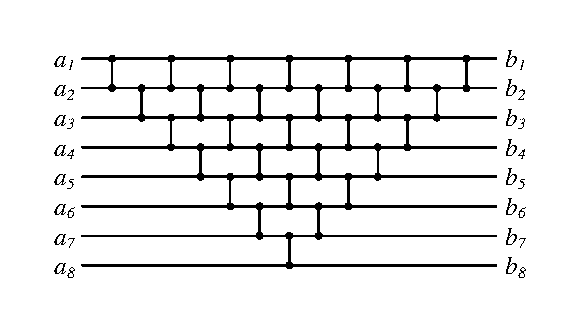
\includegraphics[width=0.4\textwidth]{img/Fig-Transposition.pdf}
    \caption{A Transposition Network Example}\label{Fig-Transposition}
\end{figure}

\begin{enumerate}
\item Prove that a transposition network with $n$ inputs is a sorting network if and only if it sorts the sequence $\langle n, n-1, \cdots, 1 \rangle$. {\color{blue}(Hint: Use an induction argument analogous to the \emph{Domain Conversion Lemma}.)}
\item {\color{red}{(Optional Sub-question with Bonus)}} Given any $n \in \mathbb{N}$, write a program using Tkinter in Python to draw a figure similar to Fig.~\ref{Fig-Transposition} with $n$ input wires.
\end{enumerate}
\begin{solution}
    \begin{enumerate}
        \item It is trival that a transposition network with $n$ inputs is a sorting network, which could sort the sequence $\langle n, n-1, \cdots, 1 \rangle$. Now, it is to be proved that if a transposition network with $n$ inputs sorts the sequence $\langle n, n-1, \cdots, 1 \rangle$ into $\langle 1,2, \cdots, n\rangle$, then it is a sorting network, i.e., a comparison network for which the output sequence $\langle b_1, b_2, \cdots, b_n \rangle$ is monotonically increasing ($b_1\leq b_2 \leq \cdots \leq b_n$) for every input sequence $\langle a_1, a_2, \cdots, a_n \rangle$. \textbf{Show this by mathematical induction.}
        \begin{description}
            \item[Basic Step.] When $n=2$, the comparison network to convert $\langle 2,1\rangle$ into $\langle 1,2\rangle$ is a single comparator acrossing the two wires.
             
            \begin{tikzpicture}
\tikzstyle{bdot} = [fill=black,circle,scale=0.3];

\draw (-3,1.5) -- (0,1.5);
\draw (-3,0.5) -- (0,0.5);
\node [bdot] (v1) at (-1.5,1.5) {};
\node [bdot] (v2) at (-1.5,0.5) {};
\draw  (v1) edge (v2);
\end{tikzpicture}
 

            According to the definition of a comparator, if the input wires are $a_i$ and $a_j$, the upper output wire always transmits $\min\{a_i,a_j\}$, and the lower output wire always transmits $\max\{a_i,a_j\}$. So it could sort any input sequence which is of size 2.
            \item[Hypothesis.] For size $k$, if the comparsion network is capable of sorting $\langle k,k-1,\cdots,1\rangle$ into $\langle 1,2,\cdots, k\rangle$, then it could sort any input sequence $\langle a_1,a_2,\cdots,a_k\rangle$ into a monotonically increasing sequence $\langle b_1,b_2,\cdots,b_k\rangle$.
            \item[Induction.] For size $k+1$, if the comparator network is capable of sorting $\langle k+1,k,\cdots,1\rangle$ into $\langle 1,2,\cdots,k+1\rangle$, then there must be a structure sorting $\langle k+1,k,\cdots, 2\rangle$ or $\langle k,k-1,\cdots,1\rangle$ because of the final result, and another sending structure to send the remaining element into the target place. 
            
            Because the property of the transposition network, to send the remaining element (1 or $k+1$ repectively) into the other end target place (the uppermost wire or the lowest wire respectively), the sending structure will come across \textbf{all the wires} in the path. The four possiblities are shown in the Figure \ref{fours} (the sending structure here is \emph{the best case structure}), which enumerates all the scenarios to be the proof for having a sub-sorting network and a sending structure.

            \begin{figure}[h]
                \centering
                \subfigure[]{\begin{tikzpicture}[scale=0.8,every node/.style={scale=0.8}]
\tikzstyle{bdot} = [fill=black,circle,scale=0.3];
\draw  (-2.5,0) node[left] {$k+1$} -- (4.5,0) node[right] {$1$};
\draw (-2.5,-1) node[left] {$\vdots$}-- (4.5,-1) node[right] {$\vdots$};
\draw (-2.5,-2) node[left] {$2$}-- (4.5,-2) node[right] {$k$};
\draw (-2.5,-3) node[left] {$1$}-- (4.5,-3) node[right] {$k+1$};

\draw[fill=white]  (-1.5,0.5) rectangle (1.5,-2.5);
\node[text width=2cm,text centered] at (0,-1) {$k$ sorting network};
\draw (2.5,-3) node [bdot] {} -- (2.5,-2) node [bdot] {};
\draw (3,-2) node [bdot] {} -- (3,-1) node [bdot] {};
\draw (3.5,-1) node [bdot] {} -- (3.5,0) node [bdot] {};




\end{tikzpicture}\label{ex}}
                \subfigure[]{\begin{tikzpicture}[scale=0.8,every node/.style={scale=0.8}]
\tikzstyle{bdot} = [fill=black,circle,scale=0.3];
\draw  (-2.5,0) node[left] {$k+1$} -- (4.5,0) node[right] {$1$};
\draw (-2.5,-1) node[left] {$\vdots$}-- (4.5,-1) node[right] {$\vdots$};
\draw (-2.5,-2) node[left] {$2$}-- (4.5,-2) node[right] {$k$};
\draw (-2.5,-3) node[left] {$1$}-- (4.5,-3) node[right] {$k+1$};

\draw[fill=white]  (0.4,-0.6) rectangle (3.4,-3.6);
\node[text width=2cm,text centered] at (1.9,-2.1) {$k$ sorting network};
\draw (-1.5,-3) node [bdot] {} -- (-1.5,-2) node [bdot] {};
\draw (-1,-2) node [bdot] {} -- (-1,-1) node [bdot] {};
\draw (-0.5,-1) node [bdot] {} -- (-0.5,0) node [bdot] {};
\end{tikzpicture}\label{k2}}
                \subfigure[]{\begin{tikzpicture}[scale=0.8,every node/.style={scale=0.8}]
\tikzstyle{bdot} = [fill=black,circle,scale=0.3];
\draw  (-2.5,0) node[left] {$k+1$} -- (4.5,0) node[right] {$1$};
\draw (-2.5,-1) node[left] {$\vdots$}-- (4.5,-1) node[right] {$\vdots$};
\draw (-2.5,-2) node[left] {$2$}-- (4.5,-2) node[right] {$k$};
\draw (-2.5,-3) node[left] {$1$}-- (4.5,-3) node[right] {$k+1$};

\draw[fill=white]  (-1.5,-0.5) rectangle (1.5,-3.5);
\node[text width=2cm,text centered] at (0,-2) {$k$ sorting network};
\draw (2.5,0) node [bdot] {} -- (2.5,-1) node [bdot] {};
\draw (3,-1) node [bdot] {} -- (3,-2) node [bdot] {};
\draw (3.5,-2) node [bdot] {} -- (3.5,-3) node [bdot] {};




\end{tikzpicture}\label{k3}}
                \subfigure[]{\begin{tikzpicture}[scale=0.8,every node/.style={scale=0.8}]
\tikzstyle{bdot} = [fill=black,circle,scale=0.3];
\draw  (-2.5,0) node[left] {$k+1$} -- (4.5,0) node[right] {$1$};
\draw (-2.5,-1) node[left] {$\vdots$}-- (4.5,-1) node[right] {$\vdots$};
\draw (-2.5,-2) node[left] {$2$}-- (4.5,-2) node[right] {$k$};
\draw (-2.5,-3) node[left] {$1$}-- (4.5,-3) node[right] {$k+1$};

\draw[fill=white]  (0.5,0.5) rectangle (3.5,-2.5);
\node[text width=2cm,text centered] at (2,-1) {$k$ sorting network};
\draw (-1.5,0) node [bdot] {} -- (-1.5,-1) node [bdot] {};
\draw (-1,-1) node [bdot] {} -- (-1,-2) node [bdot] {};
\draw (-0.5,-2) node [bdot] {} -- (-0.5,-3) node [bdot] {};




\end{tikzpicture}
\label{k4}}
                \caption{Four scenarios for size $k+1$}
                \label{fours}
            \end{figure}

            As a matter of fact, because such comparison network presereve the output order if the input order is the same according to the Domain Conversion Lemma where a monotonically increase function could be constructed, the sorting comparison networks for $\langle k,k-1,\cdots,1 \rangle$ and $\langle k+1,k,\cdots,2\rangle$ will have \textbf{the same property} for sorting any abitrary input sequence $\langle a_1,a_2,\cdots,a_k\rangle$, so they are all denoted as ``$k$ sorting network'' in the figure.

            For the network in Figure \ref{ex}, if an abitrary input sequence $\langle a_1,\cdots,a_k,x\rangle$ is put into the network, by the property of the ``$k$ sorting network'', the output for this sub-sorting structure is $\langle b_1,b_2,\cdots, b_k\rangle$ where $b_1\leq b_2\leq b_k$. And then $x$ could be placed into \textbf{the appropriate position} and the sequence is perfectly ordered. The procedure is shown in Figure \ref{k1x}. And it is similar to the network in Figure \ref{k2}, \ref{k3}, \ref{k4}. 

            \begin{figure}[H]
                \centering
                \begin{tikzpicture}[scale=0.8,every node/.style={scale=0.8}]
\tikzstyle{bdot} = [fill=black,circle,scale=0.3];
\draw  (-2.5,0) node[left] {$a_1$} -- (4.5,0) node[right] {$b_1$};
\draw (-2.5,-1) node[left] {$\vdots$}-- (4.5,-1) node[right] {$\vdots$};
\draw (-2.5,-2) node[left] {$a_k$}-- (4.5,-2) node[right] {$x$};
\draw (-2.5,-3) node[left] {$x$}-- (4.5,-3) node[right] {$b_k$};

\draw[fill=white]  (-1.5,0.5) rectangle (1.5,-2.5);
\node[text width=2cm,text centered] at (0,-1) {$k$ sorting network};
\draw (2.5,-3) node [bdot] {} -- (2.5,-2) node [bdot] {};
\draw (3,-2) node [bdot] {} -- (3,-1) node [bdot] {};
\draw (3.5,-1) node [bdot] {} -- (3.5,0) node [bdot] {};

\node at (2,0.2) {$b_1$};
\node at (2,-0.6) {$\vdots$};
\node at (2,-1.8) {$b_k$};
\node at (2,-2.8) {$x$};
\end{tikzpicture}
                \caption{Input an abitrary sequence into the network}
                \label{k1x}
            \end{figure}

            So for size $k+1$, the proposition also holds.
            \item[Conclusion.] By the principle of mathematical induction, if a transposition network with $n$ inputs sorts the sequence $\langle n, n-1, \cdots, 1 \rangle$, then it is a sorting network.
        \end{description}

        As a result, a transposition network with $n$ inputs is a sorting network $\Leftrightarrow$ it sorts the sequence $\langle n, n-1, \cdots, 1 \rangle$.
        
        % A stronger statement is here to be proved in order to prove the original proposition.

        % \begin{definition}[the order function]
        %     Stable-sorting the input sequence $\langle a_1,a_2,\cdots,a_i,\cdots,a_n\rangle$ into the sorted position numbered $\langle 1,2,\cdots, n\rangle$, the order function $f(i)$ is the target position number for $a_i$. 
        % \end{definition}

        % In a word, $f(i)$ is the order number for $a_i$ in the input sequence $\mathbf{a}$. The stable sorting here means if $a_i=a_j$ and $i<j$, then $f(i)<f(j)$, which just makes sure there is only one possible value for the every $f(i)$. The context above indicates that $f$ is a 
        
        % An exmaple: 
        % \fbox{8}\fbox{9}\fbox{6}\fbox{5} $\rightarrow$ \fbox{5}\fbox{6}\fbox{8}\fbox{9}, then $f(1)=3,f(2)=4,f(3)=1,f(4)=2$. Another example with the same numbers in the array: \fbox{8}\fbox{8}\fbox{6}\fbox{5} $\rightarrow$ \fbox{5}\fbox{6}\fbox{8}\fbox{8}, then $f(1)=3,f(2)=4,f(3)=2,f(4)=1$.

        % \begin{lemma}
        %     The 
        % \end{lemma}

        \item \fname{Code-Transposition.py} uses the construction method of Figure \ref{k4} to create the $n=8$ and $n=24$ transposition networks, which is shown in Figure \ref{tkinter}.
        \begin{figure}[H]
            \centering
            \subfigure[$n=8$]{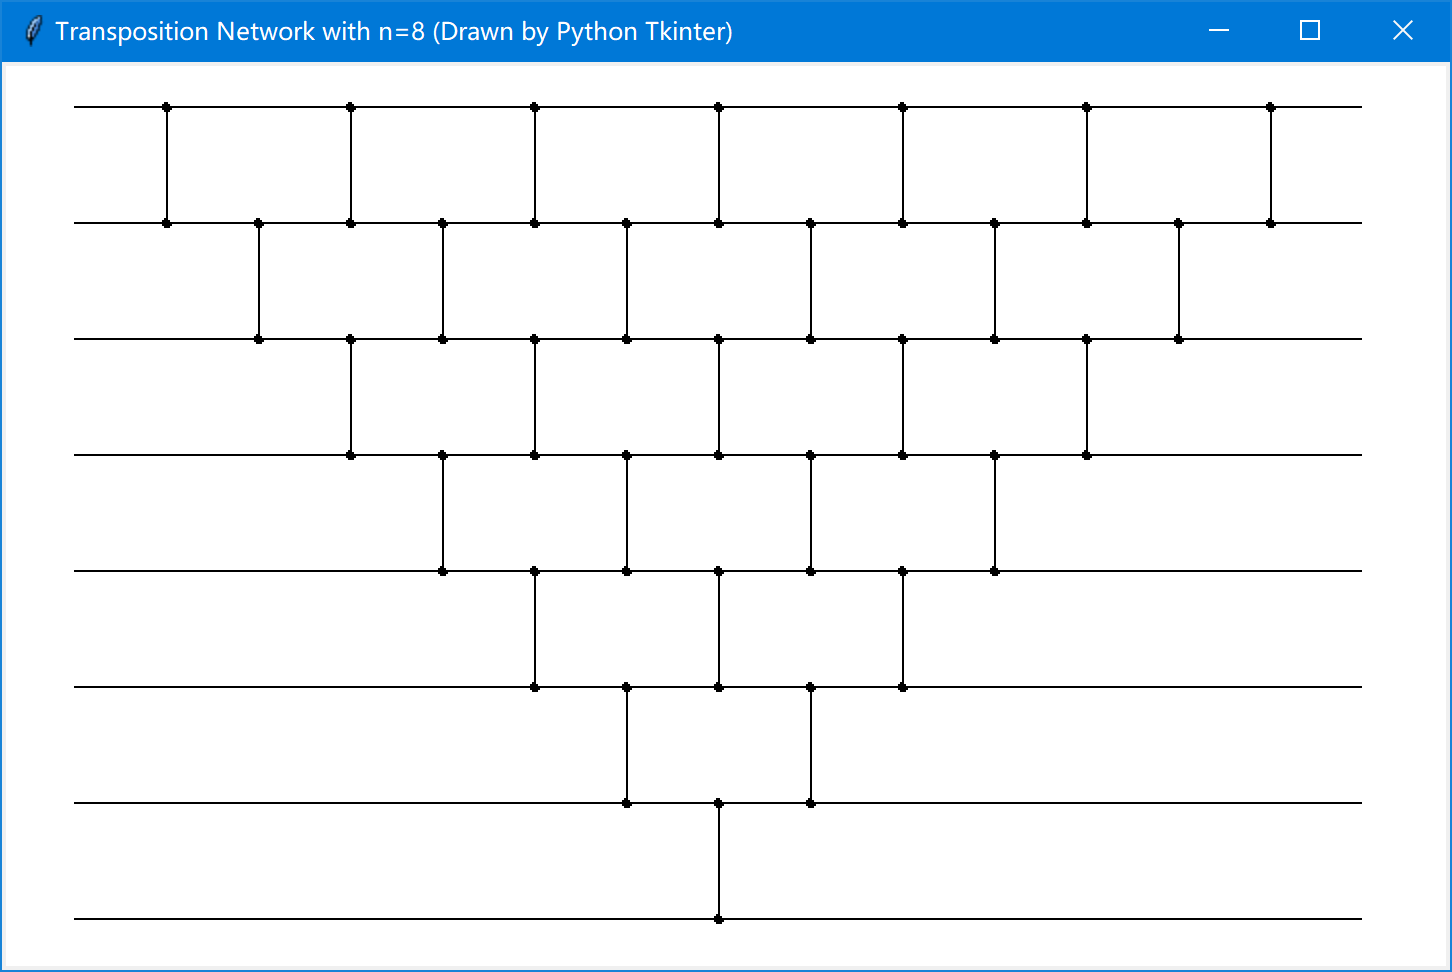
\includegraphics[height=5cm]{img/tkinter8.png}}
            \subfigure[$n=24$]{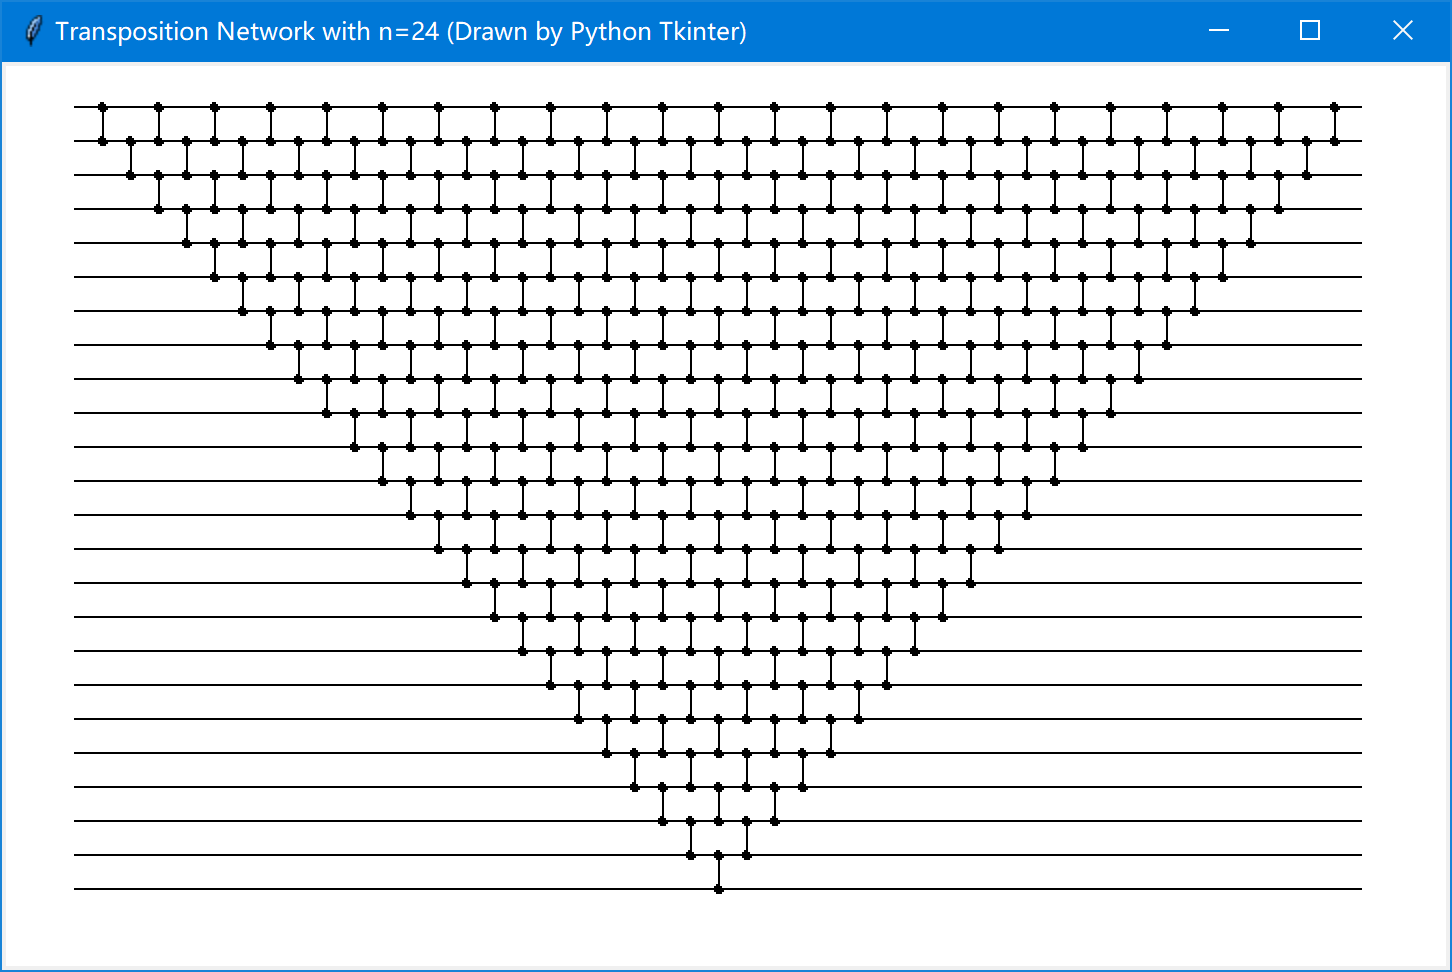
\includegraphics[height=5cm]{img/tkinter24.png}}
            \caption{Tkinter graphics of the transposition networks}
            \label{tkinter}
        \end{figure}

        \fname{Code-Transposition.py}
        \inputminted[highlightlines={47}]{Python}{code/Code-Transposition.py}
    \end{enumerate}
\end{solution}
\end{enumerate}

%========================================================================
\end{document}
